\section{SuperNEMO Tracker Extent and Energy}
\label{app:raw-observations}

For an event with $h_i$ raw tracker-hit positions $\vec{r}_{ij}$ in
millimeters, we measure spatial extent by
\begin{equation}
 R_{g,i}=\left[\frac{1}{h_i}\sum_j
 \|\vec{r}_{ij}-\overline{\vec{r}}_i\|^2\right]^{1/2},
 \qquad \overline{\vec{r}}_i=\frac{1}{h_i}\sum_j\vec{r}_{ij}.
\end{equation}
This radius of gyration uses all stored tracker hit centers with equal
weights; it is not a fitted track length. Reconstructed energy is the
calorimeter sum $E_1+E_2$, counted once per event. We retain all 262,144
$^{214}$Bi and 196,608 $0\nu\beta\beta$ test events, with no missing
energies or coordinate summaries.

Figure~\ref{fig:sn-extent-population} compares complete populations.
Each 100\,keV energy column is normalized over all 20\,mm extent bins.
Columns with fewer than 20 events are masked, affecting one $^{214}$Bi
and 35 $0\nu\beta\beta$ events. Extents above 800\,mm remain in the
normalization but are outside the heatmap view; the cumulative plots
include their full tails. These display bins are separate from EnergyBench
matching bins.

To compare balanced cohorts, events are ranked by energy and then event
ordinal within each physical class. We take the first and last quarter:
65,536 events per cohort for $^{214}$Bi and 49,152 for $0\nu\beta\beta$.
Exact energy ties are split by ordinal, not geometry. The $^{214}$Bi
quartile boundaries are 1003.0 and 1870.25\,keV; the $0\nu\beta\beta$
boundaries are 2583.125 and 2821.5\,keV. These relative energy cohorts
are not common absolute windows across classes.

Median $R_g$ decreases from 335.97 to 291.14\,mm for the illustrative
$0\nu\beta\beta$ sample and changes from 281.97 to 294.04\,mm for
$^{214}$Bi. The distributions overlap substantially. Geometry can
therefore contain energy-associated information, but these observations
do not establish its use by a trained classifier or a universal
monotonic size--energy relation. No specific physical or selection
mechanism is inferred. The formal SuperNEMO benchmark remains
$2\nu\beta\beta$ versus $^{214}$Bi.

The current point adapters center events, quantize at 15\,mm, and divide
coordinates by a fixed 1000\,mm scale; CNNs use a fixed 44\,mm occupancy
grid. They exclude calorimeter energies and do not normalize each event
to unit spatial extent. Quantization and aggregation nevertheless change
the input, so the raw extent statistic is not a claim about the learned
representation.

\begin{figure}[!htb]
\centering
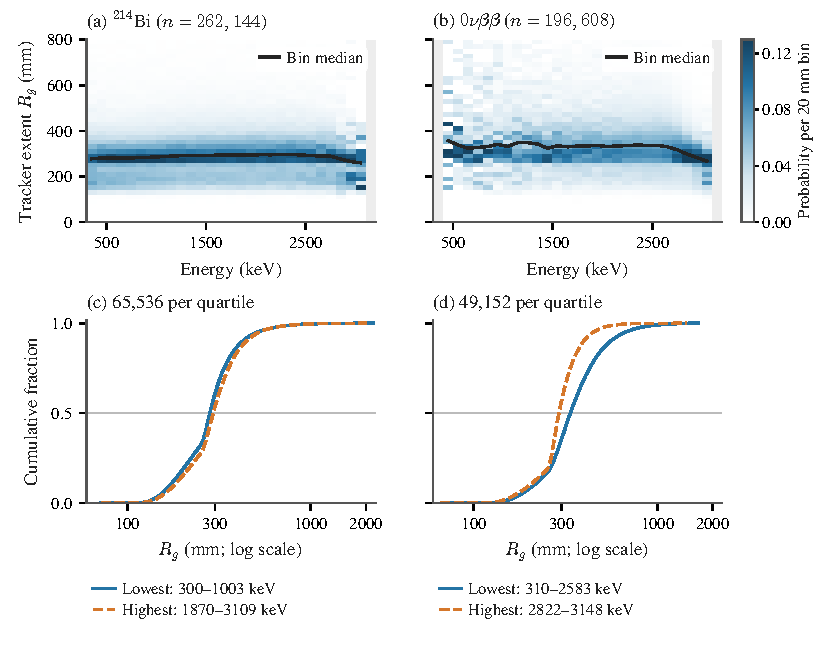
\includegraphics[width=\linewidth]{wing_contribution/figures/supernemo_extent_energy_population.pdf}
\caption{SuperNEMO tracker extent versus reconstructed energy.
Top: conditional distributions using 100\,keV by 20\,mm bins; each
energy column is normalized over all extents. Black curves show medians;
gray columns contain fewer than 20 events. Extents above 800\,mm
(0.99\% of $^{214}$Bi and 1.10\% of $0\nu\beta\beta$) are excluded from
view only. Bottom: complete cumulative distributions for the lowest
and highest energy-ranked quartiles within each class, on a logarithmic
extent axis. Cohort sizes and energy ranges are given in the panels.}
\label{fig:sn-extent-population}
\end{figure}
